\documentclass[12pt]{article}
\usepackage[utf8]{inputenc}
\usepackage{graphicx}
\usepackage[a4paper,width=150mm,top=25mm,bottom=25mm]{geometry}

\title{

\\
{COS 301 User Manual}
}



\author{Ctrl Alt Defeat}

\begin{document}

\begin{titlepage}
    \centering



    \vspace{2cm}
    \hrulefill\\
    \vspace{1cm}
    {\Huge\bfseries SRS Documentation v3.0}

    \vspace{1cm}

    {\Large Software Requirements Specification Document for\\Domain Pulse}\\
    \vspace{1cm}
    \hrulefill\\

    \vfill

    {\large Ctrl Alt Defeat}

    \vspace{1cm}

    {\large 2023/07/31}\\
    %    \vspace{1cm}
    %    \vspace{1cm}
    %    
\includegraphics[width=10cm]{../../Images/dpLogo.png}
    %    \vspace{1cm}\\
    %    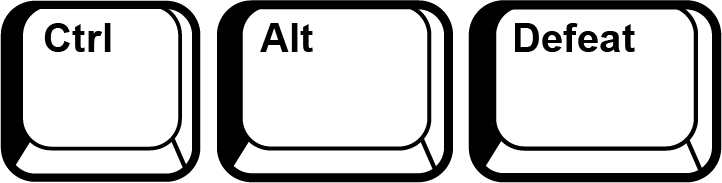
\includegraphics[width=6cm]{../../Images/cadLogo.png}

\end{titlepage}



\tableofcontents

\newpage



\section{Introduction}
\subsection{What is Domain Pulse?}
\begin{itemize}
    \item First we need to understand what Sentiment analysis is , Sentiment analysis is the process of computationally identifying and categorizing opinions expressed in a piece of text, especially in order to determine whether the writer's attitude towards a particular topic, product, etc. is positive, negative, or neutral. Now in this being said we introduce Domain Pulse.
    \item Domain pulse is the ultimate sentiment analysis platform. It gathers and analyses online opinions about any domain, be it a business, a person, or more. With stunning visuals and easy-to-understand statistics, Domain Pulse helps you understand the online presence and sentiment for any domain.
    \item Domain Pulse presents the results in a visually stunning and easy-to-understand
    format. Our wide range of visualisations bring statistics to life, which make it a breeze
    to grasp the online presence and sentiment for any domain. Take control of
    understanding public opinion like never before with Domain Pulse.
\end{itemize}







\end{document}
